%
% File acl2019.tex
%
%% Based on the style files for ACL 2018, NAACL 2018/19, which were
%% Based on the style files for ACL-2015, with some improvements
%%  taken from the NAACL-2016 style
%% Based on the style files for ACL-2014, which were, in turn,
%% based on ACL-2013, ACL-2012, ACL-2011, ACL-2010, ACL-IJCNLP-2009,
%% EACL-2009, IJCNLP-2008...
%% Based on the style files for EACL 2006 by 
%%e.agirre@ehu.es or Sergi.Balari@uab.es
%% and that of ACL 08 by Joakim Nivre and Noah Smith

\documentclass[11pt,a4paper]{article}
\usepackage[hyperref]{acl2019}
\usepackage{times}
\usepackage{latexsym}
\usepackage{graphicx}
\usepackage{float}
\usepackage{subfig}
\usepackage{url}

\aclfinalcopy % Uncomment this line for the final submission
%\def\aclpaperid{***} %  Enter the acl Paper ID here

%\setlength\titlebox{5cm}
% You can expand the titlebox if you need extra space
% to show all the authors. Please do not make the titlebox
% smaller than 5cm (the original size); we will check this
% in the camera-ready version and ask you to change it back.

\newcommand\BibTeX{B\textsc{ib}\TeX}

\title{Instructions for NLP Coursework}

\author{Hugo Mayo \\\And
  Matt Malarkey
  \\\And Arjun Narula\\}

\date{}

\begin{document}
\maketitle

\section{Data Analysis}

There are a number of ways to judge the humour of a sentence and this is evident from the fact that people perceive humour in different ways. The dataset was created by having participants apply microedits to headlines with the goal of making them funny, and as the funniness was judged by multiple people who may find different things funny, it’s worth considering what all the different strategies are that generate humour in general life and also in headlines. 

Being a dataset of headlines, it makes sense that there will probably be some key themes that exist in multiple headlines, as many news stories will be covering the same thing. Moreover, as the headlines are collected from the subreddits ‘r/worldnews’ and ‘r/politics’ on Reddit, it’s no surprise that a majority of headlines often deal with U.S. politics as the latter subreddit focuses on this subject. This is reflected in the dataset where we see that one of the most common words appearing in 39.11% of headlines is ‘Trump’, with the word ‘Donald’ not far behind. 

One technique for creating humour is through satire, which is often used to comment on issues with individuals or on society in general, commonly with a focus on politics. Therefore, it’s worth looking at whether headlines containing ‘Trump’ are in general funnier than others as it may be easier to generate satirical humour from these.  From our analysis, we found that the average funniness score for ‘Trump’ headlines was 1.02, which is higher than the training dataset average of 0.94, and furthermore, the proportion of ‘Trump’ headlines with a score greater than 1 was 42.38%, indicating that if a headline contains ‘Trump’, it’s likely to be funnier than if it doesn’t.

Another good way to generate humour is through context and there are a few ways this can be looked at in terms of the dataset. First of all, certain microedits may be funny because they’re related to the original word either semantically or through pronunciation. On the other hand, you could argue that if the two words are so unrelated to each other then the surrealness of the edit makes the headline funny. To check this, we looked at how the word similarity between the original and edit word correlates to the funniness, and the similarity was computed through the cosine distance of the GloVe vectors for those words. Figure \ref{fig:word_sim} shows that the score is highest when the distance is smaller, meaning that headlines are on average funnier if there is a semantic similarity between the words in the microedit. Figure \ref{fig:lev_dist} analyses the similarity between words based on their spelling and shows that the funniness of a headline isn’t determined by if two words are spelt similarly like ‘pie’ and ‘lie’. 

Finally, just as we looked at the context between the two words in the microedit, it’s worth looking at the context between the entire headline and the edited word, and in Figure \ref{fig:sent_sim}] we again see a similar trend in that the smaller the distance, the funnier the headline. Building on this, we can say that jokes often involve setting up some context before delivering a punchline, and so a reasonable hypothesis could be that as longer headlines give more room to establish a context, then the longer the headline the funnier it may be. Figure \ref{fig:headline_len} shows that actually if a headline is too short or too long then it’s unlikely to be funny, and so the headline length could be a good indicator for seeing which headlines won’t be funny, rather than which ones are the funniest. Another metric for looking at the length of a headline is the number of clause separators, shown in Figure \ref{fig:clause_sep} surprisingly follows a different trend to that of just counting the number of words. However, it still seems like it can be used as an indicator of assessing the funniness, as the lower the number of clause separators, the higher the score for that headline.

\begin{figure*}[htp]
\centering
\subfloat[Semantic word similarity\label{fig:word_sim}]{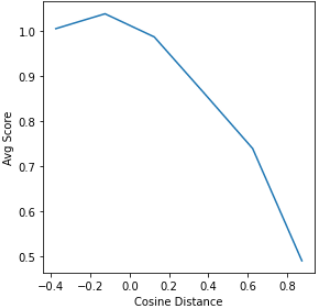
\includegraphics[width=.3\textwidth]{Graphs/DataAnalysis/cosine_distance.png}}\quad
\subfloat[Word spelling similarity\label{fig:lev_dist}]{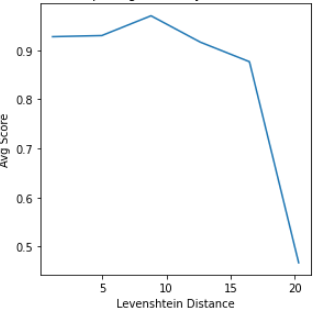
\includegraphics[width=.3\textwidth]{Graphs/DataAnalysis/levenshtein_distance.png}}\quad
\subfloat[Semantic sentence similarity\label{fig:sent_sim}]{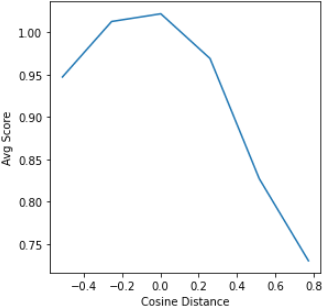
\includegraphics[width=.3\textwidth]{Graphs/DataAnalysis/cosine_sentence_distance.png}}

\medskip

\subfloat[Headline length\label{fig:headline_len}]{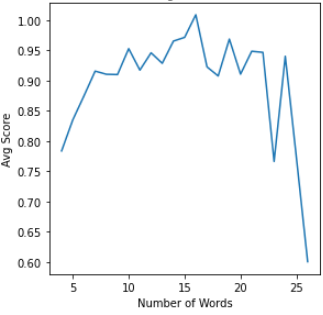
\includegraphics[width=.3\textwidth]{Graphs/DataAnalysis/headline_length.png}}\quad
\subfloat[\# of Clause Separators\label{fig:clause_sep}]{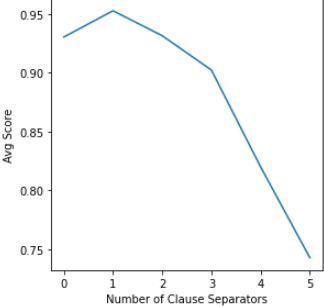
\includegraphics[width=.3\textwidth]{Graphs/DataAnalysis/clause_separator.png}}

\caption{How various metrics affect the funniness of a headline}
\label{pics:data-analysis-metrics}
\end{figure*}

\section{Approach 1}
For approach 1, we mainly considered using BERT-like models as our language models as they’re known to learn good language representations for textual data. However, before we started training our models we had to first pre-process the data. This was done in the Task1Dataset class where the headlines were tokenized, and the original word was replaced with the edit. The headline was then passed to a BERT tokenizer to encode the headlines, outputting ids and attention masks that BERT uses in training. On top of these encodings, we added extra features to each headline based on the data analysis we conducted earlier on and these are evaluated in a later section.

For our BERT models, we created a class called BertRegressionModel which can either contain a DistilBERT or RoBERTa model, as well as two linear layers. The first linear layer takes the output of the BERT model and turns it into a lower-dimensional representation which is inputted to the second layer alongside the additional features computed from the headlines. The output of the second layer is a single value representing the model’s prediction of the funniness.

Initially, DistilBERT was used as it seemed to be a quicker, more lightweight version of BERT that still retained a similar level of performance. This was good for testing training and evaluating the model, but for our final model, we chose RoBERTa simply because it has been trained on so much more data than BERT, including datasets like the CommonCrawl News dataset which may be helpful particularly as the task is looking at news headlines. However, there didn’t seem to be much of a noticeable difference in the performances of the models with both performing equally well, but with RoBERTa taking longer to train as expected. 

As it seems like the choice of the model doesn’t seem to make a huge difference, a few things that could improve the performance may be the choice of features, using more data and using an ensemble of models. From inspecting our predictions, we see that the range is only 0.177, the mean is 0.942 and the max predicted score is 1.03 which is only slightly higher than the mean of the training data. From this, it seems like the model learns how to predict a score close to the average which on average is correct. The actual scores can go up to 3.0, so it seems like with its current inputs, the model cannot predict scores that are higher than the average. Looking at the graphs from our data analysis (Figure \ref{pics:data-analysis-metrics}), this might make sense because none of our extra features can be used to distinguish between scores that are average and scores that are high, and so adding such a feature may improve the model. If in fact, the models are the issue rather than the features, than using an ensemble of different models may be useful as they’ve all been trained differently and so may recognize different and helpful characteristics in assessing the funniness.

\section{Approach 2}
\section{Feature Engineering and Evaluation}

\end{document}
